


% ----------------------------------------------------------------------------------------------- %
% ----------------------------------------------------------------------------------------------- %
\begin{frame}
\frametitle{Quantized Siren Dataset Design}
For producing quant dataset we adopted firstly Quantization Aware Training Technique known as Linear Range Quantization as described in \textit{ Benoit et al., 2018 }. More precisely,
we also levarage \textit{InteLab's Distiller} implementation of such quantazing technique, and via a configuration file called scheduler in \textit{".yaml"} format we set different
setting that we attempt for training quantized resulting models. In particular the scheduler is working around the following tunable options, which represent the degree of freedom
the technique is based on:
\begin{itemize}
\item \textbf{\textit{"Frequency"}} - it is in charge of activating distiller framework's algorithm with which update stats for carrying out quantization,
where tested frequencies have been: $[2,5,10,25]$
\item \textbf{\textit{"Per Channel"}} - it is a boolean setting that let experimenter to switch between per Layer or per Channel quantization approach, we fixed to per layer behaviour;
\item \textbf{\textit{"Weight Bits"}} - it allows us to set the number of bits with which pass from full floating-point precision to integer-precision,
where we tested: $[4,5,7,8,9,16]$ bits reduce-precision quantization;
\end{itemize}


\begin{figure}
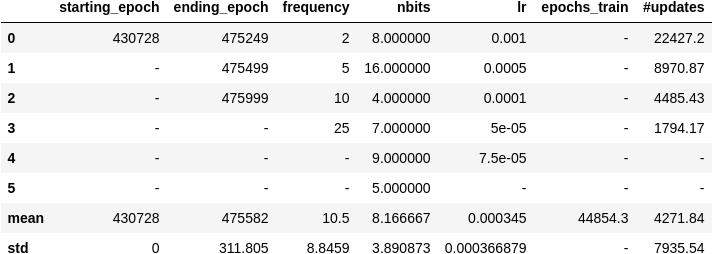
\includegraphics[scale=0.2]{slides/experiments/quant_dataset/listed_hyper_params_sets.png}
\caption{Table Hyper-Params Settings for leading Quantization Training Aware techniques as Linear Range Quantization}
\end{figure}

\end{frame}

% ----------------------------------------------------------------------------------------------- %
% ----------------------------------------------------------------------------------------------- %
\begin{frame}
\frametitle{Quantized Siren Dataset Design -  Table Hyper-params (2)}


\begin{figure}
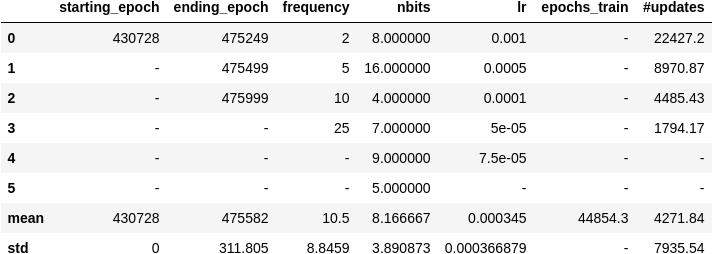
\includegraphics[scale=0.5]{slides/experiments/quant_dataset/listed_hyper_params_sets.png}
\caption{Table Hyper-Params Settings for leading Quantization Training Aware techniques as Linear Range Quantization}
\end{figure}

\end{frame}

% ----------------------------------------------------------------------------------------------- %
% ----------------------------------------------------------------------------------------------- %
\begin{frame}
\frametitle{Quantized Siren Dataset Comparing Results -  Table (1)}


\begin{figure}
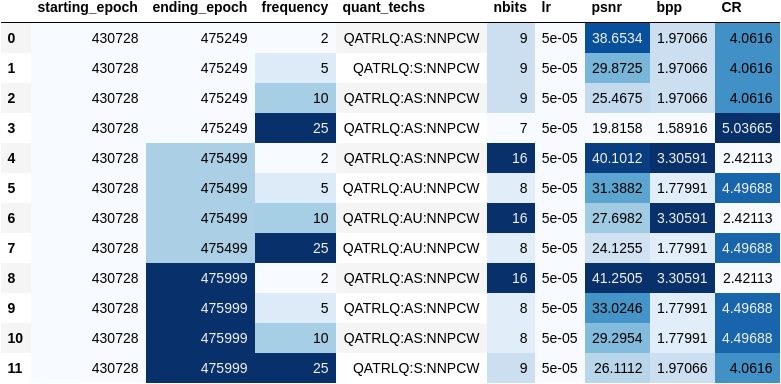
\includegraphics[scale=0.5]{slides/experiments/quant_dataset/a_table.png}
\caption{Table of just Quantization Training Aware techniques as Linear Range Quantization}
\end{figure}

\end{frame}


\begin{frame}
\frametitle{Quantized Siren Dataset Comparing Results -  Table (2)}


\begin{figure}
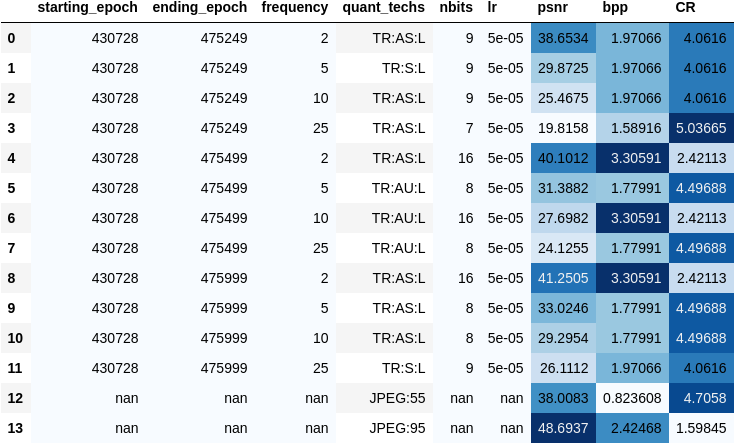
\includegraphics[scale=0.5]{slides/experiments/quant_dataset/a_table_2.png}
\caption{Table of Quantization Training Aware techniques as Linear Range Quantization compared over Jpeg}
\end{figure}

\end{frame}

% ----------------------------------------------------------------------------------------------- %
% ----------------------------------------------------------------------------------------------- %

\begin{frame}
\frametitle{Quantized Siren Dataset Current Tested Weigh Bits Choices}


\begin{figure}
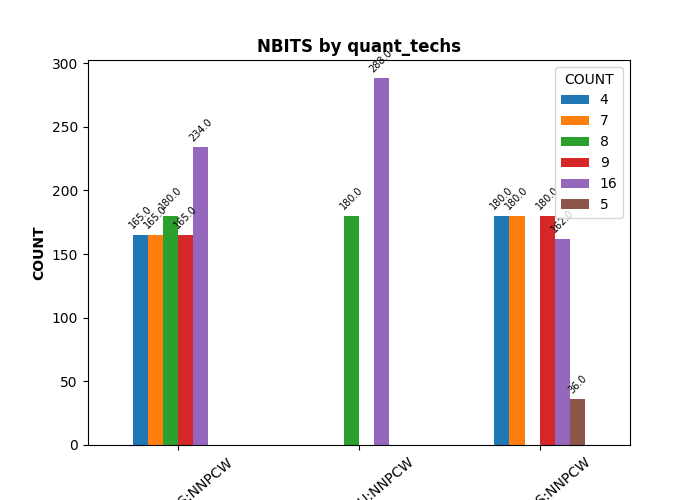
\includegraphics[scale=0.5]{slides/experiments/quant_dataset/nbits_vs_quant_techs_count_barplot.png}
\caption{Quantized Siren Dataset Current Tested Weigh Bits Choices}
\end{figure}

\end{frame}

\begin{frame}
\frametitle{Quantized Siren Dataset Comparing Results -  Scatter plot Psnr[db] vd Bpp}


\begin{figure}
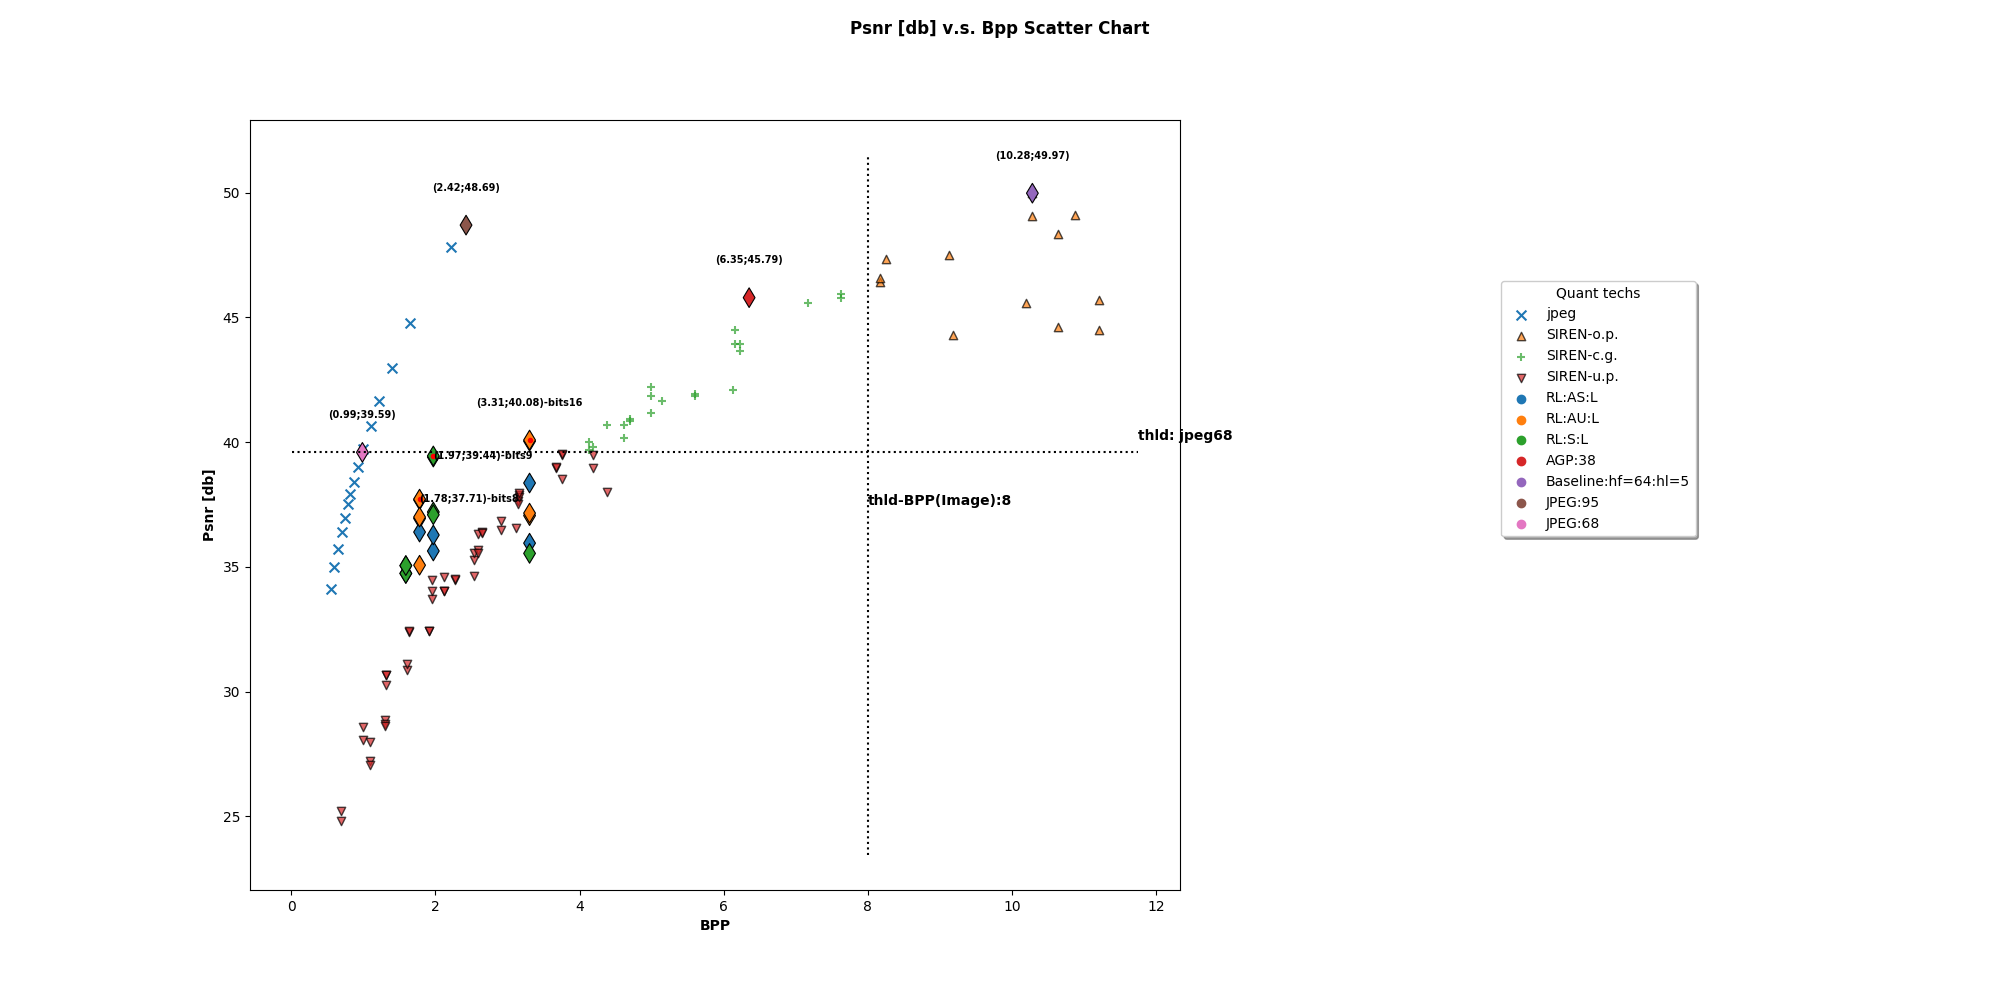
\includegraphics[scale=0.27]{slides/experiments/quant_dataset/scatter_psnr_bpp.png}
\caption{Quantized Siren Dataset Comparing Results -  Scatter plot Psnr[db] vd Bpp}
\end{figure}

\end{frame}

% ----------------------------------------------------------------------------------------------- %
% ----------------------------------------------------------------------------------------------- %
\begin{frame}
\frametitle{Quantized Siren Dataset Comparing Results -  Summary Plot}


\begin{figure}
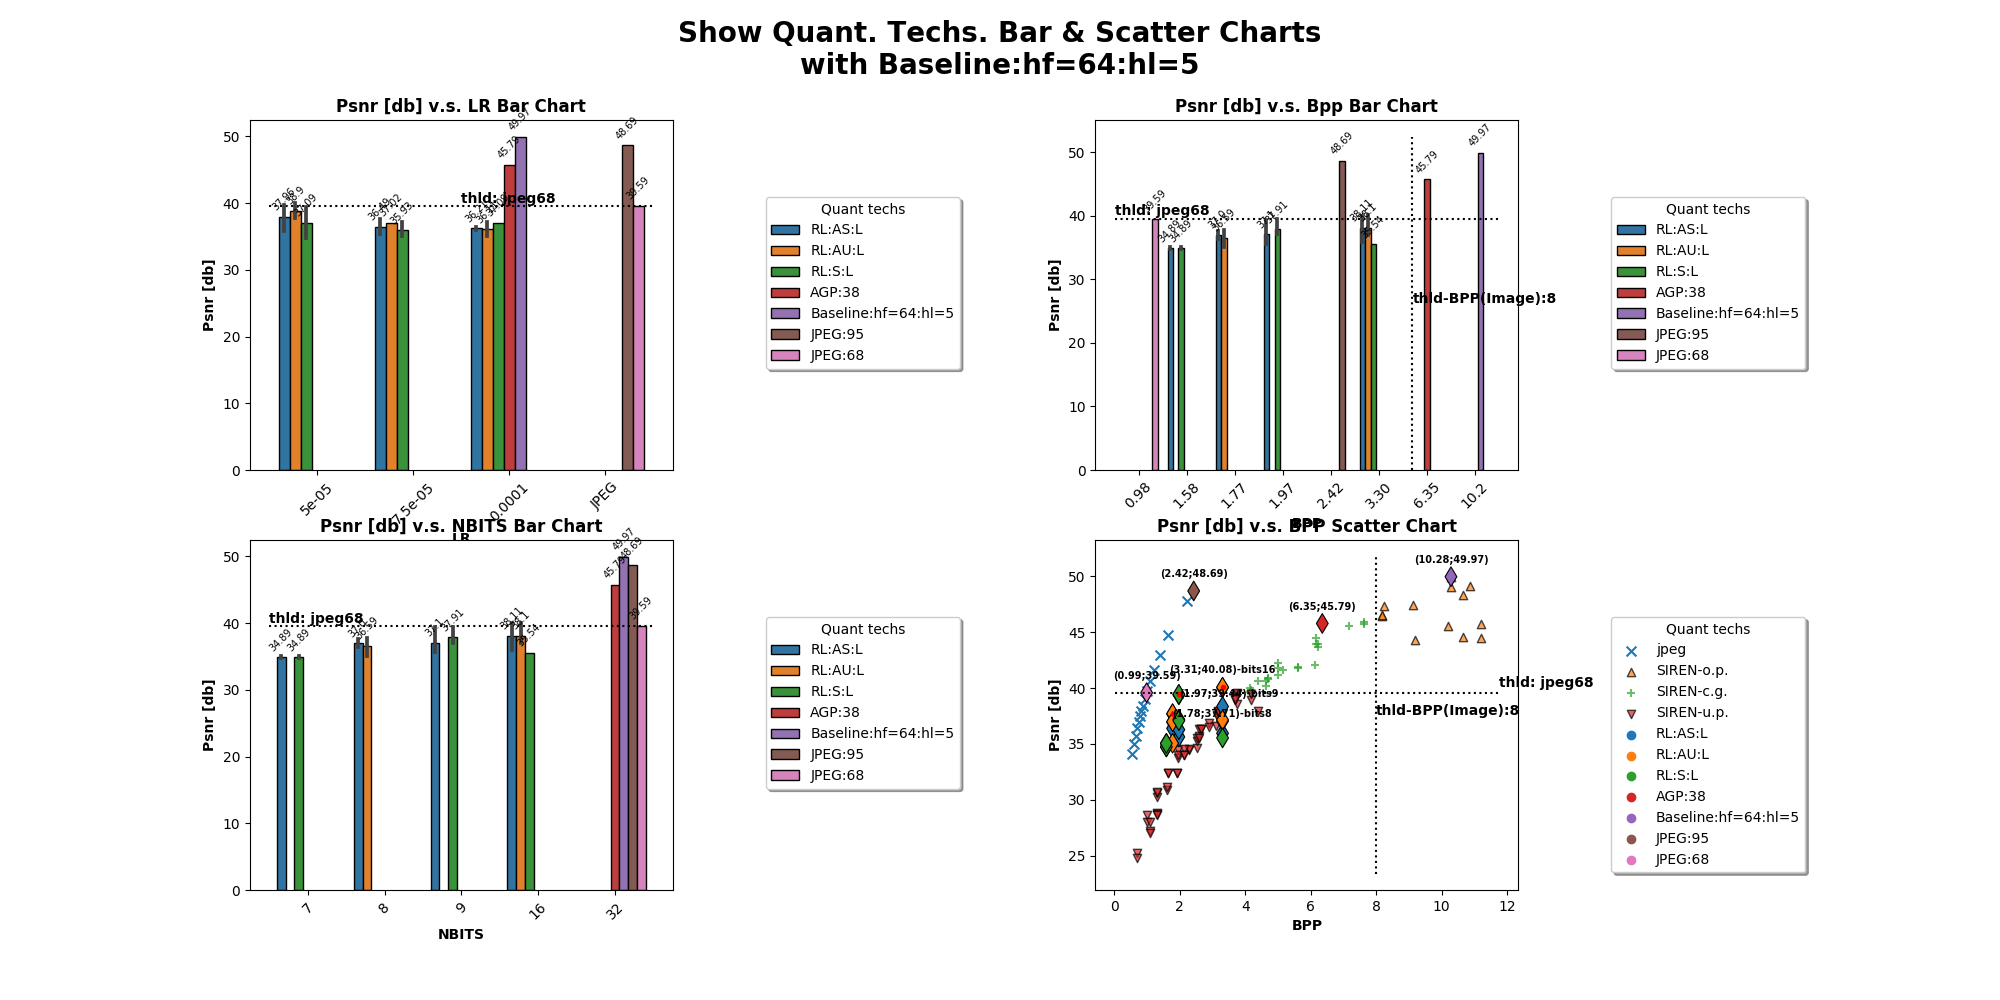
\includegraphics[scale=0.27]{slides/experiments/quant_dataset/chart_3bars_1scatter_v2.png}
\caption{Quantized Siren Dataset Comparing Results -  summary plot}
\end{figure}

\end{frame}